\documentclass[type=master]{thuthesis}
% 选项:
%   type=[bachelor|master|doctor|postdoctor], % 必选
%   secret,                                   % 可选
%   pifootnote,                               % 可选(建议打开)
%   openany|openright,                        % 可选,基本不用
%   arial,                                    % 可选,基本不用
%   arialtoc,                                 % 可选,基本不用
%   arialtitle                                % 可选,基本不用

% 所有其它可能用到的包都统一放到这里了,可以根据自己的实际添加或者删除。
\usepackage{thuthesis}

% 定义所有的图片文件在 figures 子目录下
\graphicspath{{figures/}}

% 可以在这里修改配置文件中的定义。导言区可以使用中文。
% \def\myname{薛瑞尼}

\begin{document}

%%% 封面部分
\frontmatter
\thusetup{
  %******************************
  % 注意:
  %   1. 配置里面不要出现空行
  %   2. 不需要的配置信息可以删除
  %******************************
  %
  % 中国海洋大学研究生学位论文封面
  % 参考:中国海洋大学研究生学位论文书写格式20130307.doc
  % 为避免出现错误,下面保留[清华大学学位论文模板原有定义无需修改],
  % 请直接跳到后面[中国海洋大学学位论文模板部分请根据自己情况修改]。
  %
%%%%%%%%%%%%%%%%%%%%%%[清华大学学位论文模板原有定义无需修改]%%%%%%%%%%%%%%%%%%%%%%%
  %=====
  % 秘级
  %=====
  secretlevel={秘密},
  secretyear={10},
  %
  %=========
  % 中文信息
  %=========
  ctitle={清华大学学位论文 \LaTeX\ 模板\\使用示例文档 v\version},
  cdegree={工学硕士},
  cdepartment={计算机科学与技术系},
  cmajor={计算机科学与技术},
  cauthor={薛瑞尼},
  csupervisor={郑纬民教授},
  cassosupervisor={陈文光教授}, % 副指导老师
  ccosupervisor={某某某教授}, % 联合指导老师
  % 日期自动使用当前时间,若需指定按如下方式修改:
  % cdate={超新星纪元},
  %
  % 博士后专有部分
  cfirstdiscipline={计算机科学与技术},
  cseconddiscipline={系统结构},
  postdoctordate={2009年7月——2011年7月},
  id={编号}, % 可以留空: id={},
  udc={UDC}, % 可以留空
  catalognumber={分类号}, % 可以留空
  %
  %=========
  % 英文信息
  %=========
  etitle={An Introduction to \LaTeX{} Thesis Template of Tsinghua University v\version},
  % 这块比较复杂,需要分情况讨论:
  % 1. 学术型硕士
  %    edegree:必须为Master of Arts或Master of Science(注意大小写)
  %             “哲学、文学、历史学、法学、教育学、艺术学门类,公共管理学科
  %              填写Master of Arts,其它填写Master of Science”
  %    emajor:“获得一级学科授权的学科填写一级学科名称,其它填写二级学科名称”
  % 2. 专业型硕士
  %    edegree:“填写专业学位英文名称全称”
  %    emajor:“工程硕士填写工程领域,其它专业学位不填写此项”
  % 3. 学术型博士
  %    edegree:Doctor of Philosophy(注意大小写)
  %    emajor:“获得一级学科授权的学科填写一级学科名称,其它填写二级学科名称”
  % 4. 专业型博士
  %    edegree:“填写专业学位英文名称全称”
  %    emajor:不填写此项
  edegree={Doctor of Engineering},
  emajor={Computer Science and Technology},
  eauthor={Xue Ruini},
  esupervisor={Professor Zheng Weimin},
  eassosupervisor={Chen Wenguang},
  % 日期自动生成,若需指定按如下方式修改:
  % edate={December, 2005}
  %
  % 关键词用“英文逗号”分割
  ckeywords={\TeX, \LaTeX, CJK, 模板, 论文},
  ekeywords={\TeX, \LaTeX, CJK, template, thesis}
}

% 定义中英文摘要和关键字
\begin{cabstract}
  论文的摘要是对论文研究内容和成果的高度概括。摘要应对论文所研究的问题及其研究目
  的进行描述,对研究方法和过程进行简单介绍,对研究成果和所得结论进行概括。摘要应
  具有独立性和自明性,其内容应包含与论文全文同等量的主要信息。使读者即使不阅读全
  文,通过摘要就能了解论文的总体内容和主要成果。

  论文摘要的书写应力求精确、简明。切忌写成对论文书写内容进行提要的形式,尤其要避
  免“第 1 章……;第 2 章……;……”这种或类似的陈述方式。

  本文介绍清华大学论文模板 \thuthesis{} 的使用方法。本模板符合学校的本科、硕士、
  博士论文格式要求。

  本文的创新点主要有:
  \begin{itemize}
    \item 用例子来解释模板的使用方法;
    \item 用废话来填充无关紧要的部分;
    \item 一边学习摸索一边编写新代码。
  \end{itemize}

  关键词是为了文献标引工作、用以表示全文主要内容信息的单词或术语。关键词不超过 5
  个,每个关键词中间用分号分隔。(模板作者注:关键词分隔符不用考虑,模板会自动处
  理。英文关键词同理。)
\end{cabstract}

% 如果习惯关键字跟在摘要文字后面,可以用直接命令来设置,如下:
% \ckeywords{\TeX, \LaTeX, CJK, 模板, 论文}

\begin{eabstract}
   An abstract of a dissertation is a summary and extraction of research work
   and contributions. Included in an abstract should be description of research
   topic and research objective, brief introduction to methodology and research
   process, and summarization of conclusion and contributions of the
   research. An abstract should be characterized by independence and clarity and
   carry identical information with the dissertation. It should be such that the
   general idea and major contributions of the dissertation are conveyed without
   reading the dissertation.

   An abstract should be concise and to the point. It is a misunderstanding to
   make an abstract an outline of the dissertation and words ``the first
   chapter'', ``the second chapter'' and the like should be avoided in the
   abstract.

   Key words are terms used in a dissertation for indexing, reflecting core
   information of the dissertation. An abstract may contain a maximum of 5 key
   words, with semi-colons used in between to separate one another.
\end{eabstract}

% \ekeywords{\TeX, \LaTeX, CJK, template, thesis}
%%%%%%%%%%%%%%%%%%%%%%%%%%%%%%%%%%%%%%%%%%%%%%%%%%%%%%%%%%%%%%%%%%%%%%%%%%%%%%%%

%%%%%%%%%%%%%%%%%%[中国海洋大学学位论文模板部分请根据自己情况修改]%%%%%%%%%%%%%%%%%%%
% 中国海洋大学研究生学位论文封面
% 必须填写的内容包括(其他最好不要修改):
%   分类号、密级、UDC
%   论文中文题目、作者中文姓名
%   论文答辩时间
%   封面感谢语
%   论文英文题目
%   中文摘要、中文关键词
%   英文摘要、英文关键词
%
%%%%%[自定义]%%%%%
\newcommand{\fenleihao}{}%分类号
\newcommand{\miji}{}%密级
                    % 绝密$\bigstar$20年
                    % 机密$\bigstar$10年
                    % 秘密$\bigstar$5年
\newcommand{\UDC}{}%UDC
\newcommand{\oucctitle}{基于Spring MVC架构的WEB平台系统优化策略研究}%论文中文题目
\ctitle{基于Spring MVC架构的WEB平台系统优化策略研究}%必须修改因为页眉中用到
\cauthor{武斌}%可以选择修改因为仅在 pdf 文档信息中用到
\cdegree{工学硕士}%可以选择修改因为仅在 pdf 文档信息中用到
\ckeywords{\TeX, \LaTeX, CJK, 模板, 论文}%可以选择修改因为仅在 pdf 文档信息中用到
\newcommand{\ouccauthor}{武斌}%作者中文姓名
%\newcommand{\ouccsupervisor}{姬光荣教授}%作者导师中文姓名
%\newcommand{\ouccdegree}{博\hspace{1em}士}%作者申请学位级别
%\newcommand{\ouccmajor}{海洋信息探测与处理}%作者专业名称
%\newcommand{\ouccdateday}{\CJKdigits{\the\year}年\CJKnumber{\the\month}月\CJKnumber{\the\day}日}
%\newcommand{\ouccdate}{\CJKdigits{\the\year}年\CJKnumber{\the\month}月}
\newcommand{\oucdatedefense}{2017年05月28日}%论文答辩时间
%\newcommand{\oucdatedegree}{2009年6月}%学位授予时间
\newcommand{\oucgratitude}{谨以此论文献给我的导师和亲人!}%封面感谢语
\newcommand{\oucetitle}{Research on Web Platform System Optimization Strategy Based on Spring MVC Framework}%论文英文题目
%\newcommand{\ouceauthor}{Haiyong Zheng}%作者英文姓名
\newcommand{\oucthesis}{\textsc{OUCThesis}}
%%%%%默认自定义命令%%%%%
% 空下划线定义
\newcommand{\oucblankunderline}[1]{\rule[-2pt]{#1}{.7pt}}
\newcommand{\oucunderline}[2]{\underline{\hskip #1 #2 \hskip#1}}

% 论文封面第一页
%%不需要改动%%
\vspace*{5cm}
{\xiaoer\heiti\oucgratitude

\begin{flushright}
---\hspace*{-2mm}---\hspace*{-2mm}---\hspace*{-2mm}---\hspace*{-2mm}---\hspace*{-2mm}---\hspace*{-2mm}---\hspace*{-2mm}---\hspace*{-2mm}---\hspace*{-2mm}---~\ouccauthor
\end{flushright}
}

\newpage

% 论文封面第二页
%%不需要改动%%
\vspace*{1cm}
\begin{center}
  {\xiaoer\heiti\oucctitle}
\end{center}
\vspace{10.7cm}
{\normalsize\songti
\begin{flushright}
{\renewcommand{\arraystretch}{1.3}
  \begin{tabular}{r@{}l}
    学位论文答辩日期:~ & \oucunderline{1.8em}{\oucdatedefense} \\
    指导教师签字:~ & \oucblankunderline{5cm} \\
    答辩委员会成员签字:~ & \oucblankunderline{5cm} \\
    ~ & \oucblankunderline{5cm} \\
    ~ & \oucblankunderline{5cm} \\
    ~ & \oucblankunderline{5cm} \\
    ~ & \oucblankunderline{5cm} \\
    ~ & \oucblankunderline{5cm} \\
    ~ & \oucblankunderline{5cm} \\
  \end{tabular}
}
\end{flushright}
}

\newpage

% 论文封面第三页
%%不需要改动%%
\vspace*{1cm}
\begin{center}
  {\xiaosan\heiti 独\hspace{1em}创\hspace{1em}声\hspace{1em}明}
\end{center}
\par{\normalsize\songti\parindent2em
本人声明所呈交的学位论文是本人在导师指导下进行的研究工作及取得的研究成果。据我所知,除了文中特别加以标注和致谢的地方外,论文中不包含其他人已经发表或撰写过的研究成果,也不包含未获得~\oucblankunderline{7cm}(注:如没有其他需要特别声明的,本栏可空)或其他教育机构的学位或证书使用过的材料。与我一同工作的同志对本研究所做的任何贡献均已在论文中作了明确的说明并表示谢意。
}
\vskip1.5cm
\begin{flushright}{\normalsize\songti
  学位论文作者签名:\hskip2cm 签字日期:\hskip1cm 年 \hskip0.7cm 月\hskip0.7cm 日}
\end{flushright}
\vskip.5cm
{\setlength{\unitlength}{0.1\textwidth}
  \begin{picture}(10, 0.1)
    \multiput(0,0)(0.2, 0){50}{\rule{0.15\unitlength}{.5pt}}
  \end{picture}}
\vskip1cm
\begin{center}
  {\xiaosan\heiti 学位论文版权使用授权书}
\end{center}
\par{\normalsize\songti\parindent2em
本学位论文作者完全了解学校有关保留、使用学位论文的规定,并同意以下事项:
\begin{enumerate}
\item 学校有权保留并向国家有关部门或机构送交论文的复印件和磁盘,允许论文被查阅和借阅。
\item 学校可以将学位论文的全部或部分内容编入有关数据库进行检索,可以采用影印、缩印或扫描等复制手段保存、汇编学位论文。同时授权清华大学“中国学术期刊(光盘版)电子杂志社”用于出版和编入CNKI《中国知识资源总库》,授权中国科学技术信息研究所将本学位论文收录到《中国学位论文全文数据库》。
\end{enumerate}
(保密的学位论文在解密后适用本授权书)
}
\vskip1.5cm
{\parindent0pt\normalsize\songti
学位论文作者签名:\hskip4.2cm\relax%
导师签字:\relax\hspace*{1.2cm}\\
签字日期:\hskip1cm 年\hskip0.7cm 月\hskip0.7cm 日\relax\hfill%
签字日期:\hskip1cm 年\hskip0.7cm 月\hskip0.7cm 日\relax\hspace*{1.2cm}}

\newpage

\pagestyle{plain}
\clearpage\pagenumbering{roman}

% 中文摘要
%%[需要填写:中文摘要、中文关键词]%%
\begin{center}
  {\sanhao[1.5]\heiti\oucctitle\\\vskip7pt 摘\hspace{1em}要}
\end{center}
{\normalsize\songti

  \indent
  近几年,随着中国经济的不断发展以及中国互联网整体水平的不断提高,虚拟
  经济在中国的经济发展中扮演着越来越重要的作用,WEB应用作为虚拟经济的
  主要呈现方式也获得了非常大的发展。越来越多面向不同消费群体的WEB应用
  被设计和开发出来为消费者提供各种的服务。

  随着Internet网的不断告诉发展,人们对于WEB应用的需要不再基于可用性那
  么简单,应用的用户体验越来越被重视~\cite{李梦2016基于前端的}。然而,
  随着用户数量的不断增加,WEB服务器的信息量和访问量成几何数级的增长,网
  络拥塞和服务超载日益成为开发人员必须面对的严峻问题。

  因此在WEB应用的开发过程中,开发人员不但需要在代码的书写上要进行不断优化,
  降低代码的错误率和提升代码的执行效率外,而且要将很大的精力放到服务器性能
  优化方面,通过调整WEB服务器的运行参数提升服务器的响应效率、优化缓存机制
  提升数据的存取效率,设计负载均衡方案实现应用服务器的负载均衡,开发数据库
  的主从复制和延时复制等策略保证数据的稳定性以及编写监控脚本实现服务的实施
  监控等措施来提升应用的体验和增强系统的安全性。

  本文的创新点主要有:
  \begin{itemize}
    \item 通过Jenkins实现WEB应用的自动构建和部署,提升了WEB应用的稳定性,降低代码错误率;
    \item 基于Couchbase缓存机制,加快了应用的数据读取,降低了系统的响应时间;
    \item 通过Docker容器编排技术,方便的实现服务集群节点的扩展,增强了系统的安全性,实现了统一管理和维护;
    \item 通过负载均衡,降低了应用服务器和数据服务器的压力,提升了用户的体验;
    \item 充分利用API实现监控脚本,实现了应用的实时监控,很大程度上减少了发现问题和故障处理的时间;
  \end{itemize}

}
\vskip12bp
{\xiaosi\heiti\noindent
关键词:\hskip1em Spring MVC框架应用开发; WEB应用性能优化; 数据库性能优化; 服务监控及应对方案; }

\newpage

% 英文摘要
%%[需要填写:英文摘要、英文关键词]%%
\begin{center}
  {\sanhao[1.5]\heiti\oucetitle\\\vskip7pt Abstract}
\end{center}
{\normalsize\songti

   In recent years, with the continuous development of China's economy and the continuous improvement of the overall level of China's Internet, virtual economy plays an increasingly important role in China's economic development, WEB application as a virtual economy is also the main presentation of the very Big development. More and more for different consumer groups of WEB applications are designed and developed to provide consumers with a variety of services.

   With the continuous development of the Internet to tell the people, the need for WEB applications is no longer based on usability so simple, application user experience more and more attention. However, with the increase of the number of users, the amount of information and the number of visits of the WEB server grows geometrically. Network congestion and service overload are increasingly becoming the serious problem that the developers must face.

   Therefore, in the WEB application development process, developers need to not only write code on the continuous optimization to reduce the code error rate and improve the efficiency of the code, but also to a lot of energy into the server performance optimization, By adjusting the operating parameters of the WEB server to improve the response efficiency of the server and optimize the cache mechanism to improve the efficiency of data access, the design load balancing solution to achieve the application server load balancing, database replication master and slave replication and delay replication strategy to ensure data stability As well as the preparation of monitoring scripts to achieve the implementation of service monitoring and other measures to enhance the application experience and enhance the security of the system.

   The innovation of this paper:
  \begin{itemize}
    \item Through Jenkins to realize the automatic construction and deployment of WEB applications to enhance the stability and reduce code error rate;
    \item Through Couchbase cache mechanism to speed up the data read of application, reducing the system response time;
    \item Through Docker container scheduling technology to facilitate the expansion of service cluster nodes to enhance the security of the system to achieve a unified management and maintenance;
    \item Reduces stress on application servers and data servers through load balancing and improves user experience;
    \item Make full use of API to achieve the monitoring script to achieve the application of real-time monitoring, to a large extent reduce the discovery of problems and troubleshooting time;
  \end{itemize}
}
\vskip12bp
{\xiaosi\heiti\noindent
\textbf{Keywords:\enskip WEB Aplication Development Based on Spring MVC; WEB Application Performance Optimization; Database Performance Optimization; Service Monitoring and Response Strategies}}
%%%%%%%%%%%%%%%%%%%%%%%%%%%%%%%%%%%%%%%%%%%%%%%%%%%%%%%%%%%%%%%%%%%%%%%%%%%%%%%%
% 如果使用授权说明扫描页,将可选参数中指定为扫描得到的 PDF 文件名,例如:
% \makecover[scan-auth.pdf]
\makecover

%% 目录
\tableofcontents

%% 符号对照表
\begin{denotation}[3cm]
\item[Internet] 互联网
\item[SLB] 服务器负载均衡 (Server Load Balancing)
\item[cluster] 集群
\item[Itanium] 安腾
\item[SMP] 对称多处理
\item[API] 应用程序编程接口
\item[PI] 聚酰亚胺
\item[MPI] 聚酰亚胺模型化合物,N-苯基邻苯酰亚胺
\item[PBI] 聚苯并咪唑
\item[MPBI] 聚苯并咪唑模型化合物,N-苯基苯并咪唑
\item[PY] 聚吡咙
\item[PMDA-BDA]	均苯四酸二酐与联苯四胺合成的聚吡咙薄膜
\item[$\Delta G$] 活化自由能 (Activation Free Energy)
\item[$\chi$] 传输系数 (Transmission Coefficient)
\item[$E$] 能量
\item[$m$] 质量
\item[$c$] 光速
\item[$P$] 概率
\item[$T$] 时间
\item[$v$] 速度
\end{denotation}



%%% 正文部分
\mainmatter
\chapter{绪论}
\label{cha:introduction}
\section{论文研究背景及意义}
随着信息技术的不断发展,21世纪我们已经进入了一个“信息爆炸”的社会,而且在近几年我们的社会几乎进入互联网时代后,社会中的每个人每天接收到的咨询和信息以及各种各样的互联网产品同互联网发展的初期相比,超出了太多太多。~\cite{林薇2015基于}。另外,我国的互联网技术在近十几年内不断的发展,开发WEB产品的人力成本和技术成本不断降低,用户对于 WEB 应用的需求\cite{邵志强2015跨媒体检索平台}不再满足于通过缓慢的加载和复杂的操作获取资讯~\cite{贺海梁2012基于},
许多的创业者希望通过开发一个WEB应用实现自己创业梦想的时代已经无法获得投资人的青睐。而且,由于近几年WEB信息泄露的新闻不断进入消费者的视野,用户对于WEB应用的安全性体验也提出了更高的要求。

随着互联网技术进一步普及,基于模型-视图-控制器
(Model-View-Controller, MVC)模式的WEB应用程序~\cite{张2010基于}被广大开发者所使用,目前主流的WEB应用程序均在使用此框架。使用MVC框架,可以将WEB应用进行清晰的分层开发,前端开发人员主要负责页面的呈现方式和用户体验,后台人员则主要负责应用的逻辑实现以及数据结构的搭建,极大的降低了研发成本。

随着信息化的进一步普及,数据库的使用越来越广泛,数据成为一个应用甚至也个企业最重要的价值体现,越来越多的企业发展离不开数据库。因此数据库的稳定性和安全性也称为很多企业研发的重点。通过设计数据的管理和使用机制,在提高数据库使用效率的同时,保障数据的完整性和安全性是企业运维人员的在运维过程中的重要任务。

除此之外,如何实现WEB应用的高可用性和分布式服务也是保障用户体验的一个很重要的部分,通过设计基于应用和服务器的不同层级不同纬度的优化策略,提升应用的高可用性也是在WEB应用开发中必须要注意的。

\section{国内外研究现状}
从上世纪九十年代开始,计算机技术和Internet互联网技术开始迅速发展, 随着这些技术的不断发展,在互联网络中网络信息的存储量级和访问数量都是以几何数级进行增长,随之而来导致的问题就是网络访问的拥塞问题和网络服务的超载运行~\cite{王霜2004web}。

2006年新华网被黑事件、2010年的百度域名劫持时间、2011年的CSDN用户数据泄漏事件以及2015年网易邮箱密码泄漏事件等事件无不说明系统优化的作用和意义。

目前大部分互联网产品在开始发展的阶段都重视了产品的设计和功能,然而在产品的稳定性和安全性方面却考虑不足,这在一定程度上增加了互联网产品在推广过程中潜在的风险。因此,在开发互联网产品的同时,通过一系列的优化策略,提升应用的体验,增强应用的稳定性和安全性必须得到充分的认识。

\section{论文主要研究内容}
\subsection{论文主要工作内容}
本篇论文通过在满足本人参与的WEB应用正常运行的基础上,通过应用、数据和服务等不同维度的的优化实践研究基于Spring MVC架构WEB应用的系统优化策略。首先通过搭建基于Spring MVC的WEB测试应用,在实际用户使用的过程中通过不断开发和调整系统的优化策略,提升应用的用户体验和应用的稳定性,探索行之有效的系统优化策略。

本文的研究对象主要有以下内容:

(1) 对Jenkins持续集成环境研究。自动化部署和代码检测是保证基于WEB的应用产品质量的一个重要环节,通过研究部署Jenkins集成测试环境,对编写的代码进行版本控制、自动化构建和代码测试,研究持续集成方案对于WEB应用系统优化策略的影响。

(2) 对Couchbase缓存机制进行研究。目前大多数的WEB应用对于缓存性能的优化还没有足够的重视,通过开发针对WEB应用的Couchbase缓存系统,研究Couchbase的缓存机制测试有效的缓存机制对于系统性能提升和用户体验的影响,探索可用的系统优化策略。

(3) 对Docker容器编排技术进行研究。随着用户的不断增加,单一节点的WEB应用或数据库应用已经无法满足用户的需求,如何快速的部署新的应用节点提升应用性能成为开发者关注的问题。通过构建基于Docker容器编排技术的应用容器,在新的服务器快速部署新的应用,并加入到应用集群中去,探索Docker机制对于系统优化策略的影响。

(4) 对数据库的主从复制进行研究。随着应用的发展,数据逐渐成为应用最有价值的部分,如何更好的保证数据的完整性以及安全性在应用的维护过程中日益重要。通过研究数据库的主从复制和延时复制方案,探索数据库优化对于系统安全性优化的策略。

(5) 对基于API的监控和应急措施方案进行研究。随着服务节点的不断增加,服务的高可用和服务的健康性检查时WEB应用的运维人员在维护过程中必须要注意的方面。通过开发基于API的服务器、服务监控系统以及基于API的应急处理系统研究API操作对于系统的快速检测和快速恢复的影响。

(6) 其他方面,研究WEB应用的搭建过程、Tomcat的相关配置、负载均衡以及阿里云的相关配置研究WEB应用和服务器自身优化对于系统性能的影响。

\subsection{论文目标}
本论文致力于分析目前很多WEB应用开发过程中存在的问题和不完善的地方,并探索WEB应用性能和服务器性能的优化方案。

在Linux平台上,使用JAVA语言和MySQL数据搭建一个基于Spring MVC架构的WEB应用,通过Tomcat实现应用的访问和测试,通过设计不同的优化方案对WEB进行测试,研究在实际应用中有价值的优化策略。

系统性能优化策略研究主要包含应用层面、数据层面和服务器层面三个层面。在应用层面,通过持续集成、代码审核实现应用的稳定性和安全性。在数据库层面,通过多数据库主从复制、负载均衡和备份恢复等策略实现数据的高可用和稳定性。在服务器层面,通过对服务的监控和服务器的监控、服务器间负载均衡的配置、基于API的自动化failover等策略保障服务的正常运行和高负载应对。
\section{论文组织结构}
基于Spring MVC架构WEB应用的系统优化策略的研究是按照计划逐步完成的,本人将此研究分为六个部分:

第一章:绪论。本章主要介绍WEB应用开发的现状和系统优化策略研究的意义,明确了在WEB应用开发过程中对于应用和服务器进行优化的必要性和重要性。除此之外,本章还介绍了论文主研究和实验的主要内容、论文的目标、论文创新点以及本篇论文的主要结构。

第二章:WEB应用开发介绍。本章主要介绍了前端和后端的开发框架和开发流程以及数据库的搭建过程。然后介绍了Tomcat的配置过程。之后介绍了Jenkins持续集成环境的搭建和使用过程。

第三章:应用性能优化介绍。本章主要介绍了在WEB应用性能优化方面册主要方法和策略,主要包括Couchbase缓存优化,Tomcat高性能Apr配置,Docker分布式优化以及SLB负载均衡优化等方面。同时对应用的安全性和稳定性进行了分析。

第四章:数据优化。本章主要介绍了MySQL数据库在设计和开发过程的优化策略,主要包括基于数据稳定性的复制方案,基于高可用的负载均衡方案,基于数据完整性的备份和恢复方案。同时总结了出现问题时的解决方案。

第五章:服务监控与应急措施优化。本章主要介绍了服务器层面的优化策略,主要包括多服务器的心跳监听服务配置,服务性能的监控脚本实现,基于API的应急措施处置以及服务器安全性配置等方面的优化策略。同时总结了多种方案整合使用的策略。

第六章:总结与展望。本章主要总结了不同优化策略对于系统性能的影响以及在研究过程中获得的经验,并对优化策略的进一步研究做了简单的展望。
\chapter{WEB应用开发及持续集成}
\label{cha:web}
本论文的研究目的是对于开发的WEB应用进行应用、数据库和服务器层级进行优化,通过对比不同优化策略对于系统性能提升的影响研究一套可行的系统优化策略。为了实现优化的目的,首先需要创建一个WEB应用或者对现有的应用进行优化,本人在研究生期间,参与了海信集团智能商用公司的小微商户平台系统的开发,主要工作是后台开发和服务器运维工作,因此本论文将基于参与的小微商户WEB平台进行系统优化策略的研究。

在优化之前,首先需要描述作为优化原型的小微商户WEB平台的平台的开发框架以及应用部署流程。

% 本章首先介绍WEB应用开发的主要程序语言,然后对Spring MVC框架进行了详细的介绍。同时,对各种技术的应用反问做了初步的探讨,为后文系统性能优化工作做好理论工具上的准备。
% \section{应用开发语言}
% 目前WEB应用开发主要分为前端开发和后端开发,其中前端开发以HTML和JavaScript结合为主,后端开发语言则比较多,主流的有C语言、PHP语言、JAVA语言以及Python语言等语言,不同语言之间的作用和特点都不同,但在提高系统稳定性和系统兼容性方面JAVA语言更有优势~\cite{suzumura2008performance}。
% \subsection{JAVA语言}
% \subsubsection{JAVA语言产生及发展}
% JAVA语言是在20世纪90年代产生的,任职于太阳微系统的詹姆斯·高斯林等人于1990年代初开发Java语言的雏形,最初被命名为Oak,目标设置在家用电器等小型系统的程序语言,应用在电视机、电话、闹钟、烤面包机等家用电器的控制和通信~\cite{byous1998java}。由于这些智能化家电的市场需求没有预期的高,Sun公司放弃了该项计划。随着1990年代互联网的发展,Sun公司看见Oak在互联网上应用的前景,于是改造了Oak,于1995年5月以Java的名称正式发布。Java伴随着互联网的迅猛发展而发展,逐渐成为重要的网络编程语言~\cite{java维基百科}。

% 在所有的编程语言中,应用最广泛的莫过于JAVA语言,该语言在面向对象的程序开发中一直有着突出的表现。因此在最近10几年间,JAVA语言一直保持在编程语言排行的前两名,参见图~\ref{fig:tiobe}。
% \begin{figure}[H] % use float package if you want it here
%   \centering
%   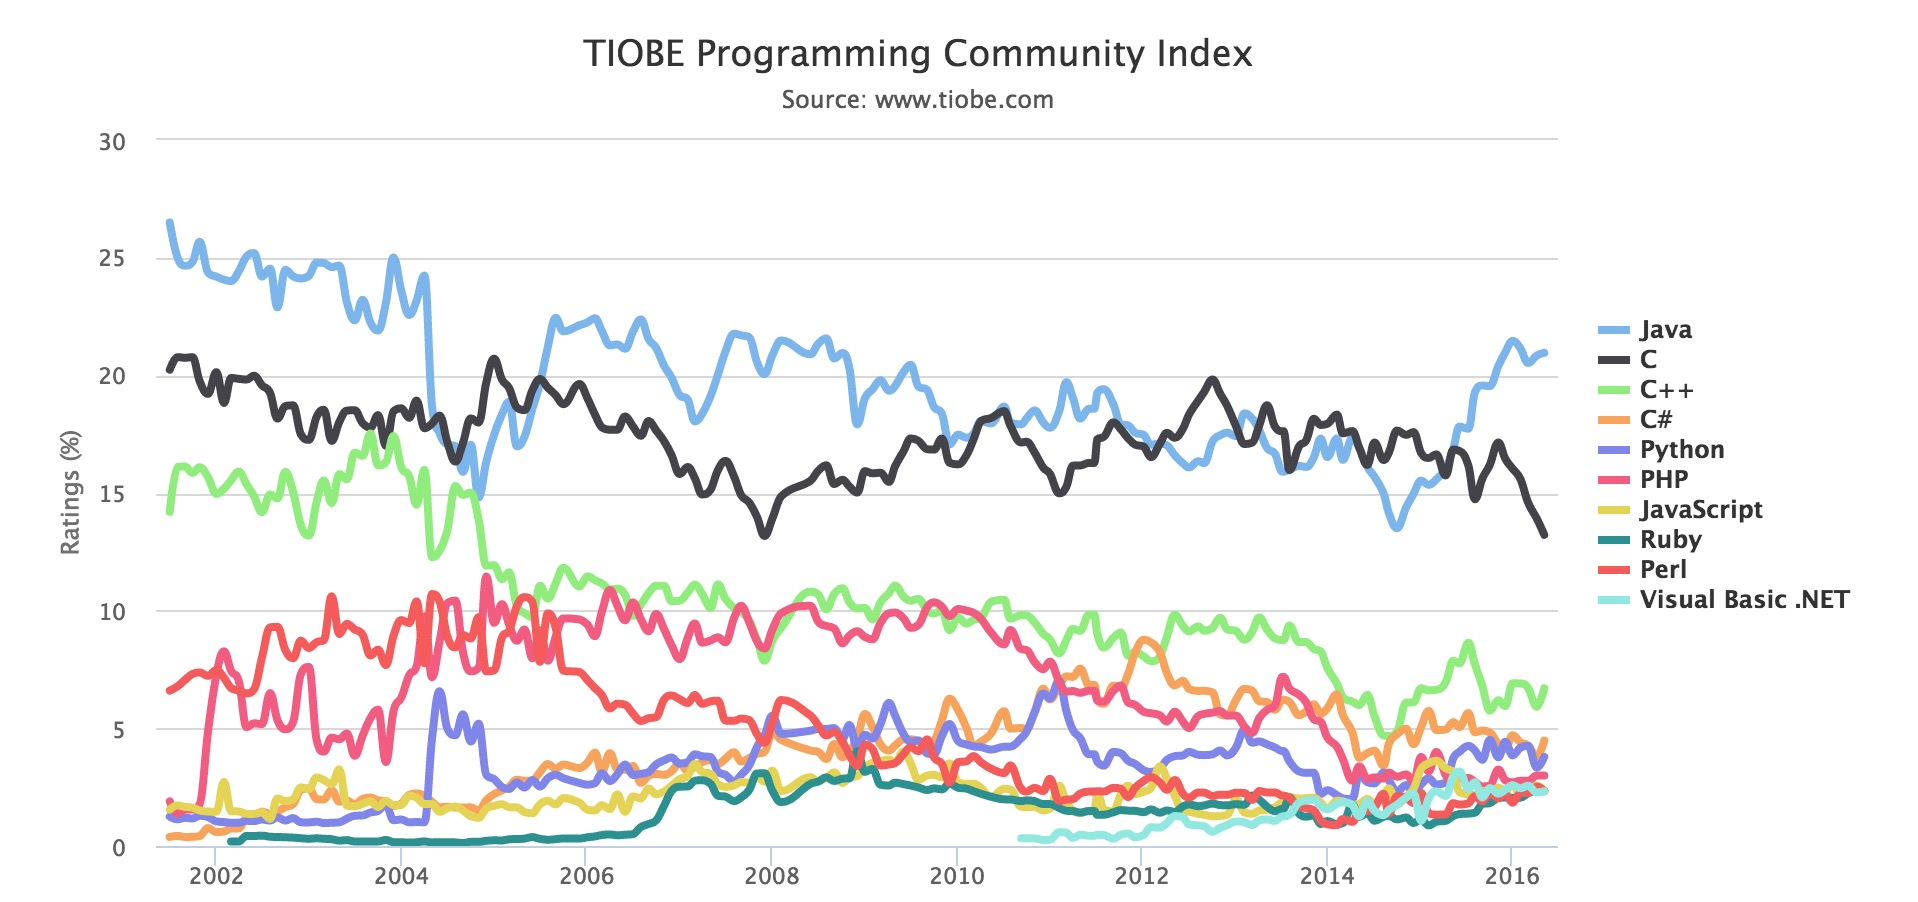
\includegraphics[width=6in]{chap02/1-TIOBE}
%   \caption{编程语言近年排行}
%   \label{fig:tiobe}
% \end{figure}
% \subsubsection{JAVA语言特点}
% 因特网的普及推动了JAVA语言的发展,同时JAVA语言在网页制作上的应用也丰富了因特网的内容。两者可谓是相辅相成、相互促进。JAVA语言的特点如表\ref{tab:java-1}。
% \begin{table}[htb]
%   \centering
%   \begin{minipage}[t]{0.8\linewidth} % 如果想在表格中使用脚注,minipage是个不错的办法
%   \caption[模板文件]{模板文件。如果表格的标题很长,那么在表格索引中就会很不美
%     观,所以要像 chapter 那样在前面用中括号写一个简短的标题。这个标题会出现在索
%     引中。}
%   \label{tab:java-1}
%     \begin{tabularx}{\linewidth}{lX}
%       \toprule[1.5pt]
%       {\heiti 特点} & {\heiti 描述} \\\midrule[1pt]
%       可移植性 & 能移植于不同的使用平台,扩大了系统的使用范围 \\
%       面向对象 & 集成了C++的优点,并且在面向对象方面有新的扩展 \\
%       多线程 & 可以让多个不同处理器同时进行工作,是数据库系统开发的最佳选择 \\
%       分布式 & 在处理TCP等协议的同时也支持网络编程\\
%       \bottomrule[1.5pt]
%     \end{tabularx}
%   \end{minipage}
% \end{table}


\section{Spring MVC开发框架}

Spring MVC 开发框架是一种针对Java语言开发的WEB系统架构,该框架的设计理念是的开发的系统整体进行分解,通过不同的方式对分解后的工作进行处理,以更加专业的技术解决具体的问题,最中在不同的模块中通过调用实现系统的整体呈现,通过这种方法系统的耦合度同其他的框架如Struts相比大大的降低。\cite{林薇2015基于}。
% \subsection{Spring MVC 架构的特点}
% Spring MVC 架构不同于传统的体系架构,在其发展的过程中吸收其他系统的特点,如支持Userful风格,灵活的本地化等。这些特征保证了Spring MVC框架在发展过程中,更加受到开发者的青睐。同时,吸收了前人的经验以后,Spring MVC框架也具备专属的特点,比如用Spring MVC框架设计的WEB系统其耦合度较低,系统总体表现出简洁明了的风格,这样用户就能更快捷的掌握数据库系统的操作~\cite{林薇2015基于}。

% Spring MVC框架是在Spring框架的基础上发展起来的,因此Spring MVC框架集成了Spring 框架的所有功能,而且两者在相互继承方面表现出很好的融合性。这一特点给系统开发带来了很多方便。除此之外,Spring MVC模型在图形兼容性和数据验证的灵活性上都有先天的优势。正式因为这些特点,使Spring MVC模型在实际应用中发挥出巨大的优势,同时也在程序员中受到青睐。本文的WEB应用就是建立在该框架之上的\cite{林薇2015基于}。
\subsection{Spring MVC 框架处理流程}

本框架是一个基于用户请求的系统架构。框架的处理过程参见图~\ref{fig:mvc},图形反映了一个简单的从用户请求开始到获得响应的过程。

\begin{figure}[H] % use float package if you want it here
  \centering
  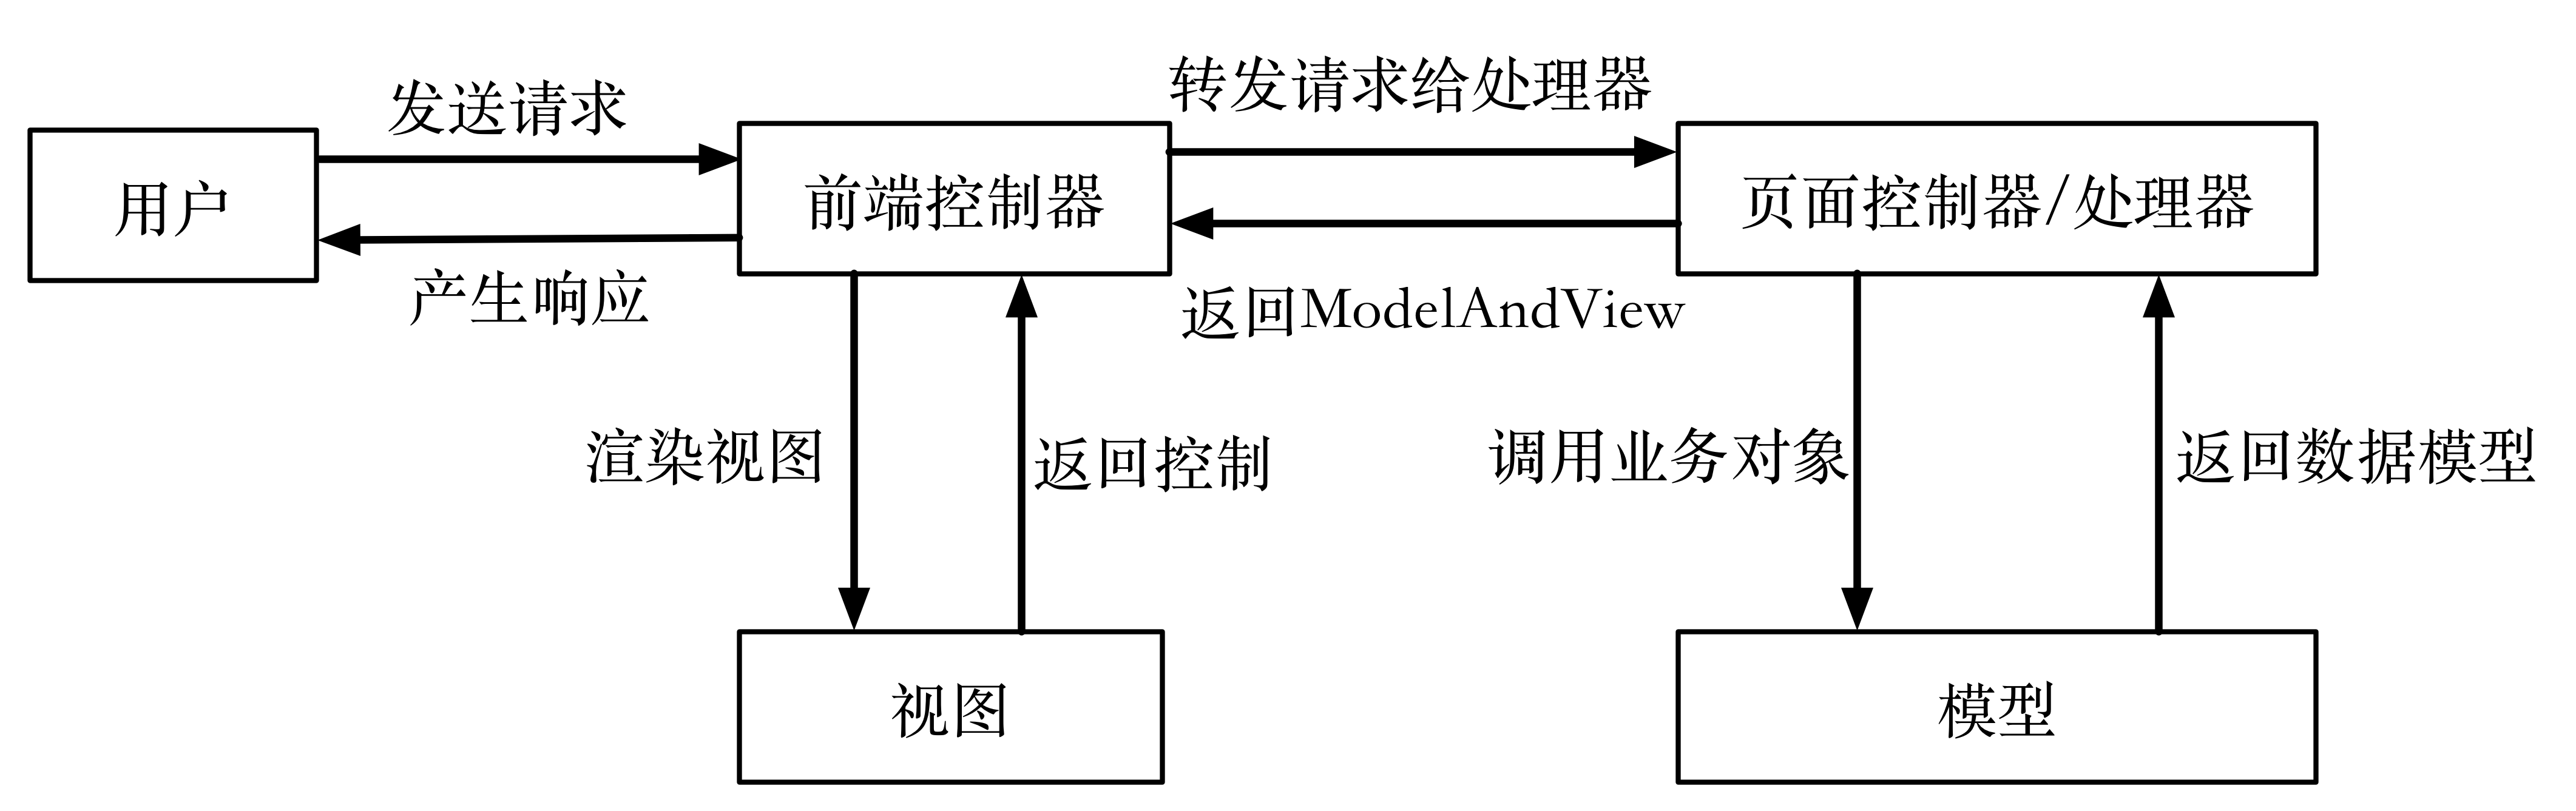
\includegraphics[width=6in]{chap02/mvc}
  \caption{Spring MVC请求响应过程}
  \label{fig:mvc}
\end{figure}

通过图可以看出,首先需要用户发送请求到框架的前端控制器,前端控制器接收到用户请求后会对用户的请求内容进行分析,获取到请求的控制器地址和请求参数,根据请求地址将用户请求转发到对应的后端控制器即处理器;处理器在接收到请求的参数之后开始调用后台的业务对象对请求进行分析和处理,在处理过程中会通过模型对存在数据库中的数据进行增、删、改、查的操作,处理完毕后将最新的数据返回给处理器;在请求的处理工作完成返回给前端控制器,之后对需要显示的结果进行视图渲染生成显示页面,展示给用户,对用户的请求产生了响应\cite{李守振2006web}。

\subsection{Spring MVC体系的三层架构}
Spring MVC开发框架的架构主要体现在MVC(Model View Controller),它是模型(M)、视图(V)和控制(C)三个英文单词的首字母缩写,根据字面意思我们也可以本系统的架构分为模型层(数据访问层)、视图层和控制层三层。

\begin{enumerate}

\item 视图层。主要负责前端页面的用户请求,将用户请求按照URL Mapping方式映射到相对应的控制器,通过分析用户请求,Spring可以自动的去寻找响应该请求的控制类,当控制类处理完请求后会将请求的结果以用户指定方式显示在前端页面上。

\item 控制层。 控制层是架构中承上启下的一层,这一层的作用是接受视图层传来的用户请求,然后针对请求设计实现用户请求的方法,需要用到数据的则会通过模型层获取数据结果,经过方法的处理获得用户请求的结果,并且将结果返回视图层。

\item 模型层,也可以成为数据访问层。这一层的作用主要是实现数据的访问方法和数据的返回方法,通过配置数据模型访问数据库并且获得需要的数据,将数据返回给控制层。

\end{enumerate}

以上的Spring MVC三层架构体系在很大程度上根据开发需求实现了业务的剥离,解决了开发过程中的开发资源和业务资源混乱的问题,而且降低了系统的耦合度。

\section{应用开发工具}

在开发基于 Spring MVC 的 WEB 应用过程中,需要用到的基础编程语言是 JAVA,系统的架构采用的 MVC 三层架构。但是在架构之外,程序本身的开发对于开发人员也非常重要,因此通过选择和使用一些比较好用的软件和工具,对于缩短开发周期提升开发效率来说非常重要。

\subsection{IntelliJ IDEA}

IntelliJ IDEA 是一款 Java 集中开发环境工具软件,由捷克软件公司 JetBrains 发布和维护~\cite{jemerov2008implementing}。

随着用户数量的增加和软件自身的优良特性,目前以及成为Java语言开发过程中效率最好的集成开发环境之一。由于它本身已经集成和非常多的使用功能和快捷键,因此在开发人员的使用过程中几乎可以摆脱鼠标,而且开发效率不降反升~\cite{IDEA维基百科}。

\subsection{Maven}

Apache Maven是由Apache软件基金会所提供德一个项目管理及自动构建工具~\cite{smart2005introduction}。它基于项目对象模型概念、能够实现一个Java项目的构建和依赖管理。本论文所涉及的WEB应用就是使用Maven来构建Java Web项目。

\subsection{Tomcat}

WEB 应用的 Web 服务器采用的是由 Apache 软件基金会 (Apache Software Foundation)开发的一个Servlet 容器,由于其本身也包含一个 HTTP 服务器,因此也常常被用作一个单独的 Web 服务器~\cite{brittain2007tomcat}。Tomcat7 支持最新 的 Servlet 3.0 规范,而且技术先进、稳定性强,最重要的一点就是免费,因此获得了众多Java语言开发者的喜欢和中时,渐渐的已经成为主流的Web应用服务器之一。

\subsection{MySQL}

MySQl是个小型关系型数据库管理系统,之所以使用MySQL是因为MySQL是一款免费的数据库管理系统,而且其建议的操作以及其兼容性都是其优点~\cite{greenspan2001mysql}。MySQL的特点主要有\cite{王川2009农业机械装备信息管理系统的设计和研究}:

\begin{itemize}

\item 为C语言、Java语言、PHP语言以及Python语言等多种编程语言提供了接口,可以实现多语言环境对MySQL数据库的调用。

\item 除了对语言的支持,MySQL还支持多线程处理,可以更加充分的利用服务器资源。

\item 除了TCP/IP协议外,还支持JDBC等多途径的数据库连接协议。

\item 除了对于数据和语言的支持外,在管理方面也有非常好的数据库管理工具,除了自己开发的Workbench还支持许多第三方工具,这些都可以对数据的数据进行管理和优化以及检查数据库的异常。

\end{itemize}

\subsection{Couchbase}

现代的互联网产品开发过程中,随着用户数量和要求的不断提高,我们需要我们的WEB产品可以同时支持更多的客户端节点并且是其保持在很低的请求延迟~\cite{brown2012getting}。为了实现这一目的,我们就需要对平台的数据开发更强大的缓存机制以提高数据的读写速度,在近几年主流的缓存系统有memcached 和 redis,虽然它们有很成熟的解决方案,但是也都有其局限性~\cite{kovacs2013cassandra}:

\begin{itemize}

\item 对于集群的支持不够好,只可以实现单个服务器的配置,不支持多服务器集群,这样就导致了在缓存扩容和负载均衡以及系统的高可用等多方面的缺点。

\item 数据持久化和故障转移表现很差,在缓存系统出现问题后修复的成本高。memcached缓存系统不支数据持持久化, redis缓存系统的持久化配置会导致服务器的负载不均衡,可能会出现间歇性负载过高的现象。

\end{itemize}

Couchbase是一个NoSQL数据库,它是世界各国的开发者在2011年推出的,由于它有良好的cluster支持、异步持久化的支持得到了众多开发者的青睐,他的特点主要有:

\begin{itemize}

\item Couchbase缓存系统对于自身的缓存配置有一个专业的WEB管理界面,除了通过页面管理,还可以通过API接口对缓存系统进行配置和管理,这些是memcached, redis 不能企及的。
\item Couchbase引入了虚拟Bucket的概念,这是建立在集群和负载均衡的基础上的,通过它可以把数据非常灵活的部署到各个集群节点中,这样对于集群就可以进行灵活的动态的管理。
\item Couchbase 的对等网设计实现了集群的负载均衡,通过智能的客户端方式可以获取集群的信息和各节点的信息,而且还支持集群节点的横向扩展。

\end{itemize}

\section{应用开发流程}

WEB应用在开发的时候设计为前后端分离,通过FDP平台实现前端到后端的请求,所以本论文测试WEB应用的开发主要分为前端开发、后端开发以及数据库搭建三个方面。

\subsection{前端开发}

应用的前端相当于MVC架构中的视图层,主要实现用户的交互,包括页面信息的展示以及用户请求的转发和响应,在前端开发中,通过Html和JavaScript来设计实现应用的页面展示,通过FDP的Ajax请求将前端的用户请求转发到应用的后端。
\subsection{后端开发}

应用的后端主要分成了Controller、Service、Pst三层,其中Controller层负责处理用户的请求然后将业务转发给Service层,Service层负责实现用户的请求,通过设计不同的业务逻辑将用户需要的数据返回,涉及到数据的读取则通过Pst层,Pst层主要负责对数据库的增删改查,将结果返回到Service层。

\subsection{数据库搭建}

应用的数据主要分为基础数据也业务数据,其中基础数据主要包括页面的功能板块、系统的定时任务、数据的权限设置、页面的功能逻辑等数据,业务数据主要包括项目使用中需要存储的商户信息和操作记录、商户的商店、商品以及销售记录等。

\section{基于Jenkins的持续集成方案开发}

在每一次WEB应用的开发、上线过程中,不可避免的要将本地环境打包上传到生产环境或者是测试环境进行解压,每一次人工的干预无疑增加了时间成本和错误率,通过Jenkis设计实现应用的持续集成,这在很大程度上能够帮助开发着实现快速的应用部署和错误重现\cite{高珺2015以持续集成方式进行系统自动化部署}。

Jenkins是一个用Java编写的开源的持续集成工具,它提供了软件开发的持续集成服务,运行在Servlet容器中,通过Jeknins可以构建基于Apache Ant 和 Apache Maven 的项目,除了构建的功能以外,Jenkins还可以执行Linux环境下的Shell命令或者脚本以及Windows环境下的bat批处理命令\cite{王宁2014基于}。

由于小微平台是通过Java语言开发的,因此可以通过Jenkins的Maven工具进行构建并进行语法检查,通过SSH插件上传构建后的war包以及前端页面到服务器端实现部署\cite{赵亚楠2013基于}。具体的自动构建及部署流程如下:

\subsection{Jenkins软件安装配置}

由于Jenkins运行在Servlet容器中,因此在安装配置Jenkins之前需要保证安装Jenkins的服务器中已经安装好了对应版本的JDK和相匹配的Tomcat软件\cite{赵杰昌2014基于}。

将Jenkins安装文件jenkins.war拷贝到运行中的Tomcat应用目录中,访问Tomcat地址完成Jenkins的相关配置后再次访问Tomcat地址进入到图\ref{fig:jenkins3}页面表示安装配置成功。

\begin{figure}[H] % use float package if you want it here
  \centering
  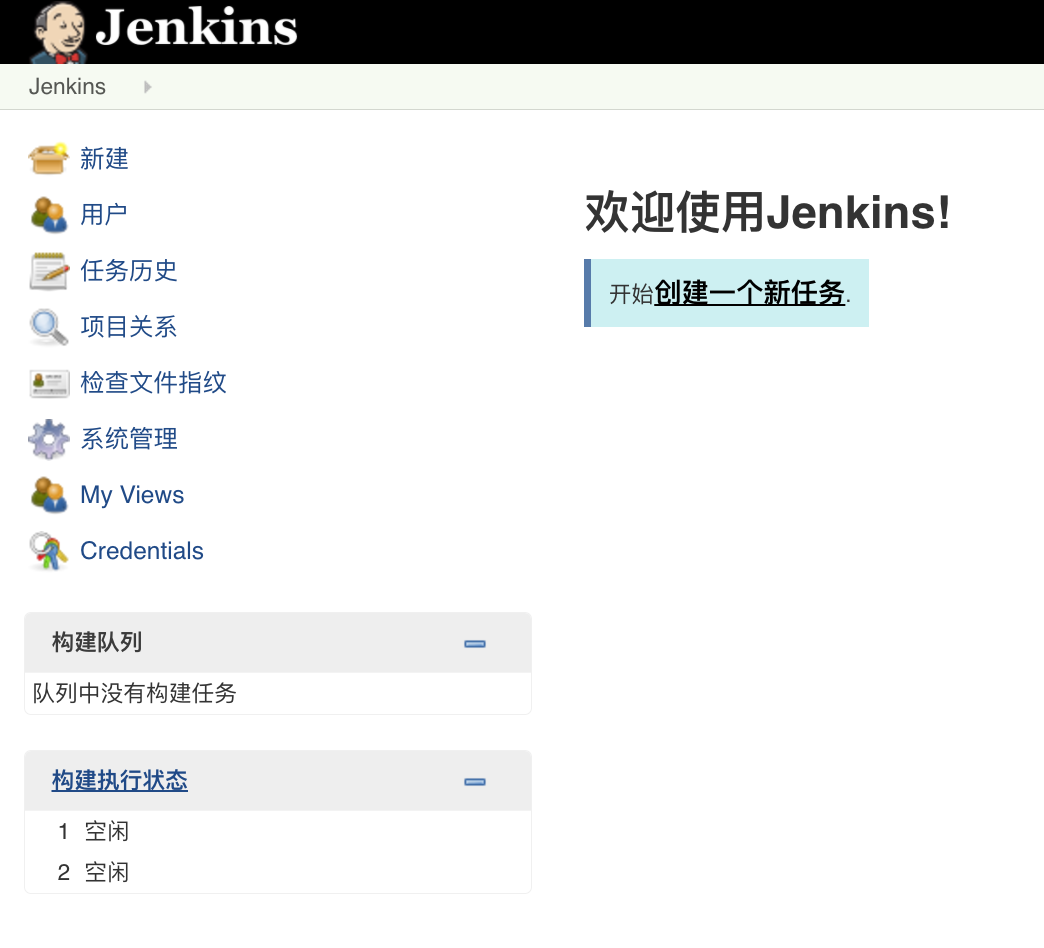
\includegraphics[width=5in]{chap02/jenkins3}
  \caption{Jenkins使用界面}
  \label{fig:jenkins3}
\end{figure}
% \begin{enumerate}
% \item 访问 http://mirrors.jenkins.io/war-stable/2.7.1/jenkins.war 下载2.7.1版本的jenkins安装包。
% \item 将jenkins.war 文件放到本地构建服务器(10.18.8.19)的Tomcat应用目录(/opt/tomcat/apache-tomcat-7.0.68/webapps)中。
% \item 配置并启动Tomcat即可完成安装,端口配置为8080,启动命令配置为:
% \begin{lstlisting}[language=bash,numbers=none]
% systemctl start/stop/status tomcat_jenkins.service
% \end{lstlisting}
% \item 访问jenkins地址(http://10.18.8.19:8080/jenkins/)初始化Jenkins:
% \begin{itemize}
% \item 完成认证,按照页面提示,将对应文件内容中的密码输入到文本框中,点击continue,如图\ref{fig:jenkins1}所示
% \begin{figure}[H] % use float package if you want it here
%   \centering
%   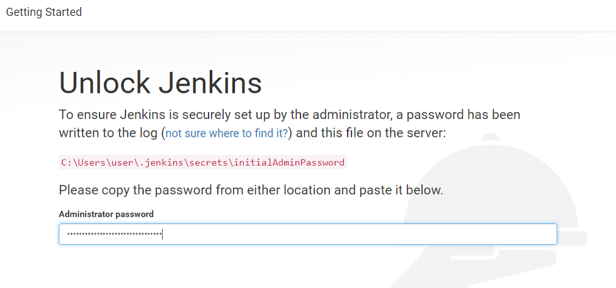
\includegraphics[width=5in]{chap02/jenkins1}
%   \caption{认证Jenkins界面}
%   \label{fig:jenkins1}
% \end{figure}
% \item 在插件选择处选择安装建议的插件
% \item 安装完成后在新的页面中配置用户名和密码完成安装,如图\ref{fig:jenkins2}
% \begin{figure}[H] % use float package if you want it here
%   \centering
%   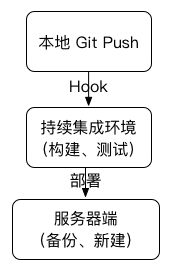
\includegraphics[width=5in]{chap02/jenkins2}
%   \caption{创建用户名和密码}
%   \label{fig:jenkins2}
% \end{figure}
% \item 进入图\ref{fig:jenkins3}页面表示安装成功
% \begin{figure}[H] % use float package if you want it here
%   \centering
%   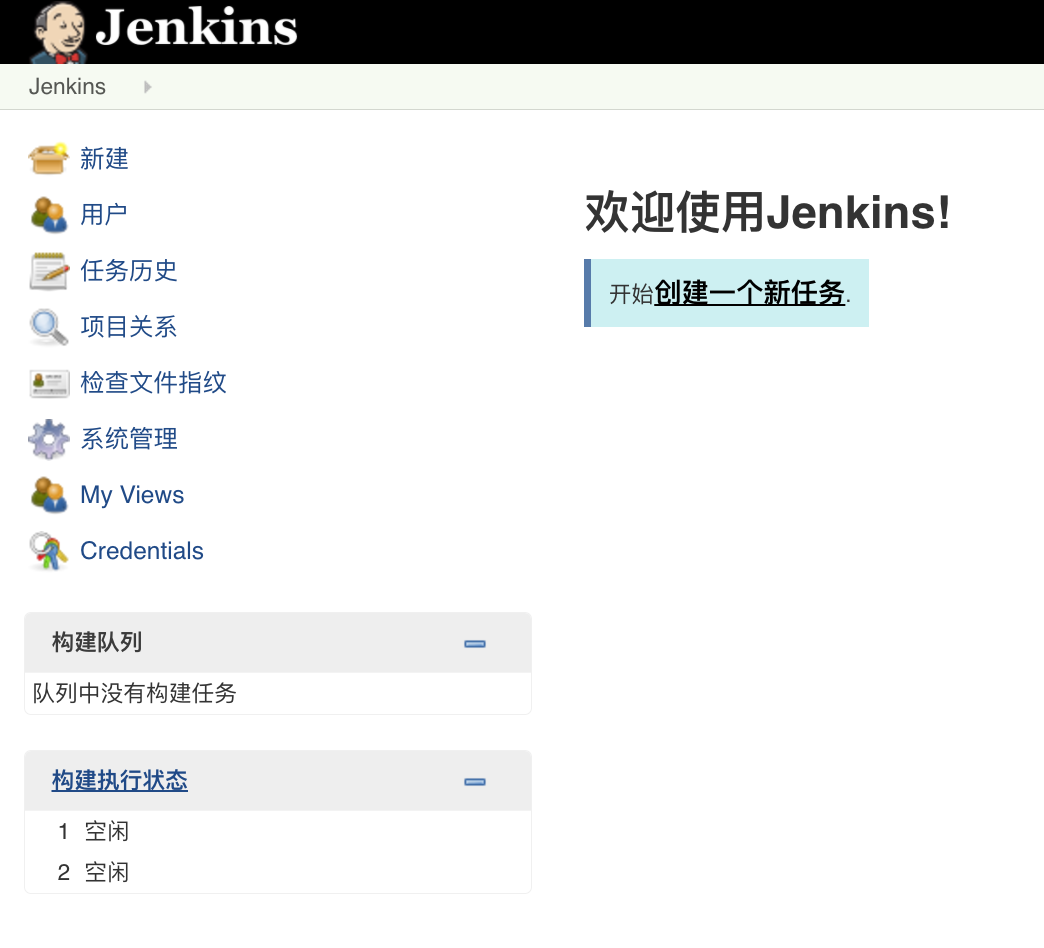
\includegraphics[width=5in]{chap02/jenkins3}
%   \caption{Jenkins使用界面}
%   \label{fig:jenkins3}
% \end{figure}
% \end{itemize}
% \end{enumerate}
\subsection{自动构建及检查方案设计}

由于小微平台通过Maven工具来解决代码使用过程中的函数依赖和本地项目构建\cite{董晓光2014使用},所以在进行自动构建的时候同样可以通过使用Maven Integration plugin插件实现项目的构建和代码检查,另外由于小微平台在开发过程中使用SVN来进行代码的版本控制,因此也需要在Jenkins中配置SVN插件来进行代码的同步和版本管理,除此之外,需要在安装Jenkins的服务器中提前安装好Maven软件。

小微项目在开发过程中通过前后端分离进行的开发,因此在构建过程中需要新建前端项目和后端项目,考虑到前端项目的构建相对后端项目比较简单,本论文只介绍后端项目的创建和构建过程。
\begin{itemize}
  \item 新建Jenkins项目
  \begin{enumerate}
    \item 在Jenkins主页面新建项目后,首先填写项目名称(以ServerDeployforPROD1.2为例)
    \item 源码管理配置为SVN,具体如图\ref{fig:jenkins4}所示:
      \begin{figure}[H] % use float package if you want it here
        \centering
        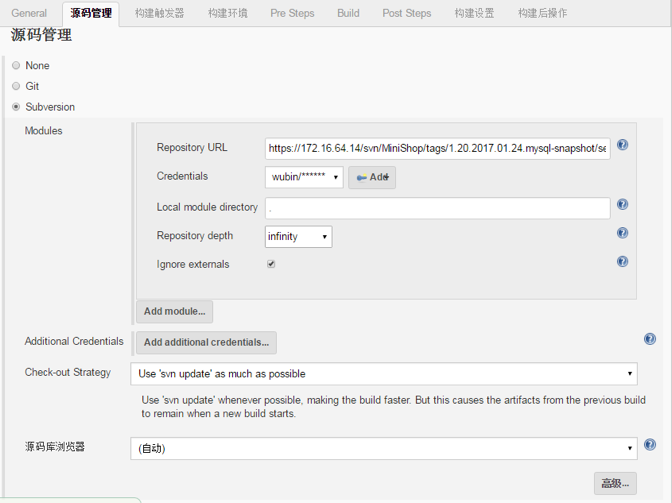
\includegraphics[width=6in]{chap02/jenkins4}
        \caption{Jenkins SVN配置}
        \label{fig:jenkins4}
      \end{figure}
      在对应的框中填写代码库的地址、通过Add按钮实现SVN的权限认证,其它选项选择默认即可。
    \item 在Pre Steps处增加shell命令为:
\begin{lstlisting}[language=bash,numbers=none]
rm -rf target/MiniShop
\end{lstlisting}
      确保每次构建时清除前一次构建信息。
    \item 在build标签页下配置构建时的操作,主要包括配置POM文件(pom.xml)的位置,pom.xml文件主要描述本Maven工程的整个生命周期所需要执行的功能和特性\cite{mileva2009mining},考虑到本项目的实际开发过程在这里选择项目pom2.xml
    \item 在Post Steps配置构建完成后的操作,首先需要在"Run only if build succeeds or is unstable"出打勾,保证在只有构建成功后才执行构建完成后的操作,其次需要配置构建完成对文件的操作:
\begin{lstlisting}[language=bash,numbers=none]
cp target/MiniShop.war /data/test/server/PROD/V1.2/MiniShop1.2_$(date +%Y%m%d)_$BUILD_NUMBER.war && chmod 777 /data/test/server/PROD/V1.2/MiniShop1.2_$(date +%Y%m%d)_$BUILD_NUMBER.war
\end{lstlisting}
      通过上述命令将每次构建完成后的文件进行备份保存和修改响应权限。
  \end{enumerate}
  所有项目信息配置完成后保存即可。
  \item 构建Jenkins项目

  进入项目主页,在页面左侧点击“立即构建”按钮即可进行构建,构建完成后将构建完成的war包上传到服务器即可,如果构建失败则表示在代码的书写过程中存在错误或者项目的库存在异常,需要在项目构建页面的构建信息页面中查看错误信息,并且根据错误信息来解决问题。
\end{itemize}

\subsection{自动部署方案设计}

Jenkins自动部署的方案是在每次构建完成后,让Jenkins可以自动的通过SSH协议访问远程服务器并将构建完成后的文件上传到服务器,并且执行服务器中的相应脚本来实现自动备份旧项目和部署新项目的目的。

\begin{enumerate}
  \item 在具体配置自动部署之前,需要先安装Publish Over SSH插件,通过这个插件,Jenkins可以实现通过SSH协议对远程服务器的访问。
  \item 在插件安装完成之后,需要配置插件来配置访问SSH的密钥和密码,在Jenkins“系统管理-系统设置”页面中会出现如图\ref{fig:jenkins5}配置:
    \begin{figure}[H] % use float package if you want it here
      \centering
      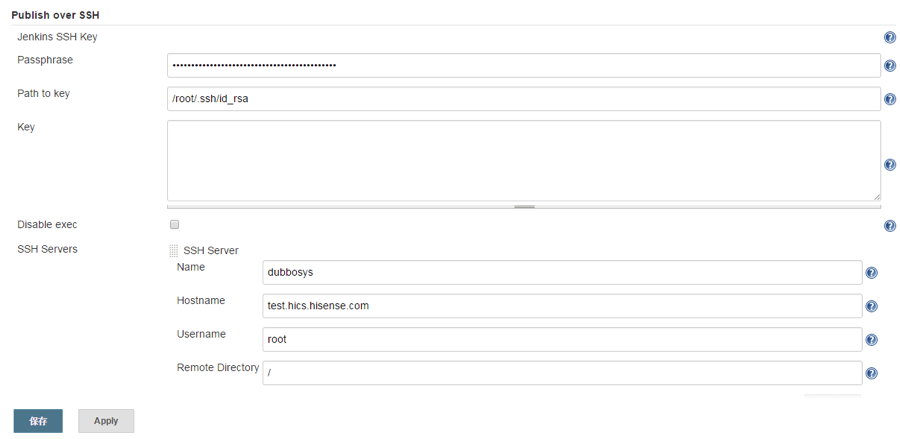
\includegraphics[width=6in]{chap02/jenkins5}
      \caption{Publish Over SSH插件配置}
      \label{fig:jenkins5}
    \end{figure}
  按照不同项目配置SSH Server信息和登录验证信息等。
  \item 插件配置完成后需要配置自动部署,插件安装完成后在“构建后操作”的选项中会出现“Send build artifacts over SSh”的选项,点击之后会出现配置:
    \begin{figure}[H] % use float package if you want it here
      \centering
      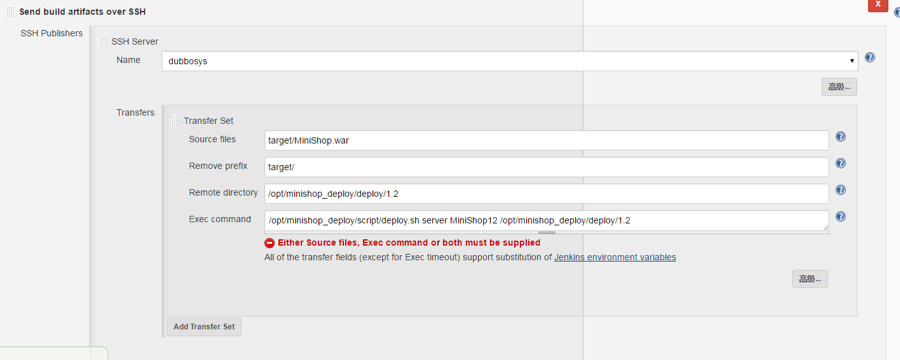
\includegraphics[width=7in]{chap02/jenkins6}
      \caption{Jenkins 自动部署配置}
      \label{fig:jenkins6}
    \end{figure}
  配置上传的文件名,上传后的路径,上传后需要执行的脚本和参数等,脚本可以参考附录\ref{cha:jenkinsdeploy}。
  \item 配置完成后再进行构建,Jenkins会自动的在构建后将构建生成的文件上传到服务器端指定路径,通过执行指定的脚本和参数将文件部署到Tomcat中,实现自动部署。
\end{enumerate}

\section{本章总结}

本章主要介绍了本人参与的小微项目的WEB平台所使用的开发框架、开发工具、开发过程以及系统上线的持续集成方案,通过持续集成方案增强了代码上线的稳定性,在本文后面的三章将会对本章开发的平台进行不通层级的优化,来实现本项目的安全性和高性能。


%%% 其它部分
\backmatter

%% 本科生要这几个索引,研究生不要。选择性留下。
% 插图索引
\listoffigures
% 表格索引
\listoftables
% 公式索引
\listofequations


%% 参考文献
% 注意:至少需要引用一篇参考文献,否则下面两行可能引起编译错误。
% 如果不需要参考文献,请将下面两行删除或注释掉。
\bibliographystyle{thuthesis}
\bibliography{ref/refs}


%% 致谢
% 如果使用声明扫描页,将可选参数指定为扫描后的 PDF 文件名,例如:
% \begin{acknowledgement}[scan-statement.pdf]
\begin{acknowledgement}
  衷心感谢导师郑海永教授副教授对本人的精心指导。他的言传身教将使
  我终生受益。

  在美国麻省理工学院化学系进行九个月的合作研究期间,承蒙 xxx 教授热心指导与帮助,不
  胜感激。感谢 xx 实验室主任 xx 教授,以及实验室全体老师和同学们的热情帮助和支
  持!本课题承蒙国家自然科学基金资助,特此致谢。

  感谢 \thuthesis,它的存在让我的论文写作轻松自在了许多,让我的论文格式规整漂亮了
  许多。
\end{acknowledgement}


%% 附录
\begin{appendix}

\chapter{其它附录}
前面两个附录主要是给本科生做例子。其它附录的内容可以放到这里,当然如果你愿意,可
以把这部分也放到独立的文件中,然后将其 \cs{input} 到主文件中。

\end{appendix}

%% 个人简历
\begin{resume}

  \resumeitem{个人简历}

  1991 年 7 月 9 日出生于 山东 省 诸城 市。

  2010 年 9 月考入 中国海洋 大学 电子 系 电子信息工程 专业,2014 年 7 月本科毕业并获得 工学 学士学位。

  2014 年 9 月免试进入 中国海洋 大学 电子 系攻读 电子与通信工程工学 学位至今。

  \researchitem{发表的学术论文} % 发表的和录用的合在一起

  % 1. 已经刊载的学术论文(本人是第一作者,或者导师为第一作者本人是第二作者)
  \begin{publications}
    \item Zheng H, Wu B, Wei T, et al. Global Exponential Robust Stability of High-Order Hopfield Neural Networks with S-Type Distributed Time Delays[J]. Journal of Applied Mathematics, 2014, 2014.
    % \item XXX, XX, Wei T, et al. Global Exponential Robust Stability of High-Order Hopfield Neural Networks with S-Type Distributed Time Delays[J]. Journal of Applied Mathematics, 2014, 2014.
  \end{publications}

\end{resume}

\end{document}
